\ifdefined\included
\else
\documentclass[a4paper,11pt,twoside]{StyleThese}
\usepackage{amsmath,amssymb, amsthm}             % AMS Math
\usepackage[T1]{fontenc}
\usepackage[utf8x]{inputenc}
\usepackage{babel}
\usepackage{datetime}

\usepackage{silence}

\WarningFilter{minitoc(hints)}{W0023}
\WarningFilter{minitoc(hints)}{W0028}
\WarningFilter{minitoc(hints)}{W0030}

\usepackage{lmodern}
\usepackage{tabularx}
%\usepackage{tabular}
\usepackage{multirow}
\usepackage{xspace}

\usepackage{hhline}
\usepackage[left=1.5in,right=1.3in,top=1.1in,bottom=1.1in,includefoot,includehead,headheight=13.6pt]{geometry}
\renewcommand{\baselinestretch}{1.05}

% Table of contents for each chapter

\usepackage[nottoc, notlof, notlot]{tocbibind}
\usepackage{minitoc}
\setcounter{minitocdepth}{2}
\mtcindent=15pt
% Use \minitoc where to put a table of contents

\usepackage{aecompl}

% Glossary / list of abbreviations

\usepackage[intoc]{nomencl}
\iftoggle{ThesisInEnglish}{%
\renewcommand{\nomname}{Glossary}
}{ %
\renewcommand{\nomname}{Liste des Abréviations}
}

\usepackage{etoolbox}
\renewcommand\nomgroup[1]{%
  \item[\bfseries
  \ifstrequal{#1}{A}{Number Sets}{%
  \ifstrequal{#1}{G}{Agents Beliefs and Action Models}{%
  \ifstrequal{#1}{N}{Navigation}{%
  \ifstrequal{#1}{O}{Ontology}{%
  \ifstrequal{#1}{R}{Referring Expression Generation}{%
  \ifstrequal{#1}{Z}{Controllable and Uncontrollable Agents Task Planning}{}}}}}}%
]}

\makenomenclature



% My pdf code

\usepackage{ifpdf}

\ifpdf
  \usepackage[pdftex]{graphicx}
  \DeclareGraphicsExtensions{.jpg}
  \usepackage[pagebackref,hyperindex=true]{hyperref}
  \usepackage{tikz}
  \usetikzlibrary{arrows,shapes,calc}
\else
  \usepackage{graphicx}
  \DeclareGraphicsExtensions{.ps,.eps}
  \usepackage[dvipdfm,pagebackref,hyperindex=true]{hyperref}
\fi

\graphicspath{{.}{images/}}

%% nicer backref links. NOTE: The flag ThesisInEnglish is used to define the
% language in the back references. Read more about it in These.tex

\iftoggle{ThesisInEnglish}{%
\renewcommand*{\backref}[1]{}
\renewcommand*{\backrefalt}[4]{%
\ifcase #1 %
(Not cited.)%
\or
(Cited in page~#2.)%
\else
(Cited in pages~#2.)%
\fi}
\renewcommand*{\backrefsep}{, }
\renewcommand*{\backreftwosep}{ and~}
\renewcommand*{\backreflastsep}{ and~}
}{%
\renewcommand*{\backref}[1]{}
\renewcommand*{\backrefalt}[4]{%
\ifcase #1 %
(Non cité.)%
\or
(Cité en page~#2.)%
\else
(Cité en pages~#2.)%
\fi}
\renewcommand*{\backrefsep}{, }
\renewcommand*{\backreftwosep}{ et~}
\renewcommand*{\backreflastsep}{ et~}
}

% Links in pdf
\usepackage{color}
\definecolor{linkcol}{rgb}{0,0,0.4} 
\definecolor{citecol}{rgb}{0.5,0,0} 
\definecolor{linkcol}{rgb}{0,0,0} 
\definecolor{citecol}{rgb}{0,0,0}
% Change this to change the informations included in the pdf file

\hypersetup
{
bookmarksopen=true,
pdftitle="Planning For Both Robot and Human: Anticipating and Accompanying Human Decisions",
pdfauthor="Guilhem BUISAN", %auteur du document
pdfsubject="Thèse", %sujet du document
%pdftoolbar=false, %barre d'outils non visible
pdfmenubar=true, %barre de menu visible
pdfhighlight=/O, %effet d'un clic sur un lien hypertexte
colorlinks=true, %couleurs sur les liens hypertextes
pdfpagemode=None, %aucun mode de page
pdfpagelayout=SinglePage, %ouverture en simple page
pdffitwindow=true, %pages ouvertes entierement dans toute la fenetre
linkcolor=linkcol, %couleur des liens hypertextes internes
citecolor=citecol, %couleur des liens pour les citations
urlcolor=linkcol %couleur des liens pour les url
}

% definitions.
% -------------------

\setcounter{secnumdepth}{3}
\setcounter{tocdepth}{2}

% Some useful commands and shortcut for maths:  partial derivative and stuff

\newcommand{\pd}[2]{\frac{\partial #1}{\partial #2}}
\def\abs{\operatorname{abs}}
\def\argmax{\operatornamewithlimits{arg\,max}}
\def\argmin{\operatornamewithlimits{arg\,min}}
\def\diag{\operatorname{Diag}}
\newcommand{\eqRef}[1]{(\ref{#1})}

\usepackage{rotating}                    % Sideways of figures & tables
%\usepackage{bibunits}
%\usepackage[sectionbib]{chapterbib}          % Cross-reference package (Natural BiB)
%\usepackage{natbib}                  % Put References at the end of each chapter
                                         % Do not put 'sectionbib' option here.
                                         % Sectionbib option in 'natbib' will do.
\usepackage{fancyhdr}                    % Fancy Header and Footer

% \usepackage{txfonts}                     % Public Times New Roman text & math font
  
%%% Fancy Header %%%%%%%%%%%%%%%%%%%%%%%%%%%%%%%%%%%%%%%%%%%%%%%%%%%%%%%%%%%%%%%%%%
% Fancy Header Style Options

\pagestyle{fancy}                       % Sets fancy header and footer
\fancyfoot{}                            % Delete current footer settings

%\renewcommand{\chaptermark}[1]{         % Lower Case Chapter marker style
%  \markboth{\chaptername\ \thechapter.\ #1}}{}} %

%\renewcommand{\sectionmark}[1]{         % Lower case Section marker style
%  \markright{\thesection.\ #1}}         %

\fancyhead[LE,RO]{\bfseries\thepage}    % Page number (boldface) in left on even
% pages and right on odd pages
\fancyhead[RE]{\bfseries\nouppercase{\leftmark}}      % Chapter in the right on even pages
\fancyhead[LO]{\bfseries\nouppercase{\rightmark}}     % Section in the left on odd pages

\let\headruleORIG\headrule
\renewcommand{\headrule}{\color{black} \headruleORIG}
\renewcommand{\headrulewidth}{1.0pt}
\usepackage{colortbl}
\arrayrulecolor{black}

\fancypagestyle{plain}{
  \fancyhead{}
  \fancyfoot{}
  \renewcommand{\headrulewidth}{0pt}
}

%\usepackage{MyAlgorithm}
%\usepackage[noend]{MyAlgorithmic}
\usepackage{algorithm}
\usepackage[noend]{algpseudocode}
\usepackage{comment}
\usepackage[ED=EDSYS-Robo, Ets=INSA]{tlsflyleaf}
%%% Clear Header %%%%%%%%%%%%%%%%%%%%%%%%%%%%%%%%%%%%%%%%%%%%%%%%%%%%%%%%%%%%%%%%%%
% Clear Header Style on the Last Empty Odd pages
\makeatletter

\def\cleardoublepage{\clearpage\if@twoside \ifodd\c@page\else%
  \hbox{}%
  \thispagestyle{empty}%              % Empty header styles
  \newpage%
  \if@twocolumn\hbox{}\newpage\fi\fi\fi}

\makeatother
 
%%%%%%%%%%%%%%%%%%%%%%%%%%%%%%%%%%%%%%%%%%%%%%%%%%%%%%%%%%%%%%%%%%%%%%%%%%%%%%% 
% Prints your review date and 'Draft Version' (From Josullvn, CS, CMU)
\newcommand{\reviewtimetoday}[2]{\special{!userdict begin
    /bop-hook{gsave 20 710 translate 45 rotate 0.8 setgray
      /Times-Roman findfont 12 scalefont setfont 0 0   moveto (#1) show
      0 -12 moveto (#2) show grestore}def end}}
% You can turn on or off this option.
% \reviewtimetoday{\today}{Draft Version}
%%%%%%%%%%%%%%%%%%%%%%%%%%%%%%%%%%%%%%%%%%%%%%%%%%%%%%%%%%%%%%%%%%%%%%%%%%%%%%% 

\newenvironment{maxime}[1]
{
\vspace*{0cm}
\hfill
\begin{minipage}{0.5\textwidth}%
%\rule[0.5ex]{\textwidth}{0.1mm}\\%
\hrulefill $\:$ {\bf #1}\\
%\vspace*{-0.25cm}
\it 
}%
{%

\hrulefill
\vspace*{0.5cm}%
\end{minipage}
}

\let\minitocORIG\minitoc
\renewcommand{\minitoc}{\minitocORIG \vspace{1.5em}}

\usepackage{multirow}
%\usepackage{slashbox}

\newenvironment{bulletList}%
{ \begin{list}%
	{$\bullet$}%
	{\setlength{\labelwidth}{25pt}%
	 \setlength{\leftmargin}{30pt}%
	 \setlength{\itemsep}{\parsep}}}%
{ \end{list} }

\theoremstyle{definition}
\newtheorem{definition}{Definition}
\renewcommand{\epsilon}{\varepsilon}

% centered page environment

\newenvironment{vcenterpage}
{\newpage\vspace*{\fill}\thispagestyle{empty}\renewcommand{\headrulewidth}{0pt}}
{\vspace*{\fill}}

\usepackage{tablefootnote}

\theoremstyle{plain}
\newtheorem{constraint}{Constraint}[section]

\algnewcommand\algorithmicforeach{\textbf{for each}}
\algnewcommand\algorithmicin{\textbf{in}}
\algdef{S}[FOR]{ForEach}[2]{\algorithmicforeach\ #1\ \algorithmicin\ #2\ \algorithmicdo}

\usepackage{listings}
\lstdefinestyle{customPlan}{
  language=C,
  commentstyle=\itshape\color{green!25!black},
}
\usepackage{pdfpages}

\sloppy
\begin{document}
\setcounter{chapter}{4} %% Numéro du chapitre précédent ;)
\dominitoc
\faketableofcontents
\fi

\chapter{Task Planner Integration With Other Component in a Complete Robotic Architecture for Human Robot Interaction}
\label{chapter:integration}
\chaptermark{Integrating Planning in an Architecture}
\minitoc

\section{Introduction}
In the last chapter, we presented a task planning approach dedicated to HRI where we not only plan for the robot but also model the human decisions, actions and reactions in order to predict and adapt to their actions and guide their decisions. This approach has been implemented on a prototype planner and be used on several examples demonstrating its strengths and drawbacks.

In this short chapter, we present how this prototype planner has been integrated in a complete robotic architecture, once again showing the versatility and usefulness of this new task planning approach. First, we detail the integration of the planner with different components of the architecture. We end this chapter by presenting a new simple yet challenging task for human robot interaction which, to our knowledge, has not been tackled by the community and for which we developed a robotic architecture, integrating our task planner, to handle it in the nominal case.

Integrating in a complete robotic architecture is obviously not only a personal work, so we want to thank two other PhD. students Guillaume Sarthou, designing and developing the ontology engine used by the planner in this chapter and Amandine Mayima designing and developing the supervision component in charge of requesting plans and using them to perform the task while managing the interaction and handling any contingencies.

\section{Integrating With Other Components}
\label{sec:chap5integratingwithothers}

Such task planning component as the one presented earlier only takes on its full meaning when integrated into a robotic architecture. Indeed, its use is quite limited if initial world states have to be set by hand in the planning domain and if the elaborated plans are not executed. In this section we describe how we integrated the planner presented in the last chapter with other components allowing to retrieve the initial states (including human beliefs) from an ontology, to match the hybrid approach presented in Chapter~\ref{chapter:comm} by using the REG component and to communicate with the supervision through ROS.

\subsection{Retrieving the Current State and Beliefs From the Knowledge Base}
Before any planning process could start, the planner must be initialized with the current world state (robot beliefs) and the estimation of the human's beliefs. To do so, we use the knowledge base presented in Chapter~\ref{chapter:comm}: the ontologies. In our architecture, each human the robot is interacting with has a dedicated ontology, fed by a perspective taking component estimating the human beliefs; in addition to the robot own ontology, representing the world state. Thus, each agent beliefs $\agentstate$ are initialized with the facts in its respective ontology.
However, ontologies can contain a lot of information that are not needed for planning, and worse, that can hamper keeping world state consistency if the planning domains do not consider some of these facts (\textit{e.g.} an action deleting a fact but not deleting the inverse relation). To cope with this issue, we define two special attributes in the world state objects: the \textit{types} and the \textit{individuals} attributes.

The \textit{types} attribute must be set by the user before retrieving the current world state. It is a dictionary linking a type name to a list of property names. A world state must be initialized solely with this attributes before being passed to a function retrieving the world state from the ontology. This function takes the agent name as the argument, and will fill the world state with the ontology matching to this name. This function fills the \textit{individuals} attribute of the world state with a dictionary linking the types specified as keys of the  \textit{types} dictionary to a list of entities/individuals inheriting from these types. Then, a world state attribute is created for each property defined in the \textit{type} attribute, and filled with a map linking a subject entity to existing entities list according to the relations in the ontology. Communication with the ontology is done using the Ontologenius~\cite{sarthou2019ontologenius} python API. For example, in the ontology from Chapter~\ref{chapter:comm} describing the siutation of Figure~\ref{fig:chap3keys}(a) represented in Figure~\ref{fig:chap3aboxtbox} and \ref{fig:chap3aboxrel}, in a domain aiming at sorting the keys collaboratively does not need to represent the color of the keys nor of the areas. In this example, the \textit{type} attribute would be set to: 

\definecolor{greenstring}{RGB}{6, 125, 23}
\definecolor{bluekeyword}{RGB}{0, 51, 179}
\definecolor{greycomment}{RGB}{140, 140, 140}
\lstset{frame=tb,
  language=Python,
  breaklines=true,
  showstringspaces=false,
  columns=flexible,
  numbers=none,
  commentstyle=\color{greenstring},
  stringstyle=\color{greenstring},
  basicstyle=\small\tt,
  keywordstyle=\color{bluekeyword},
  commentstyle=\color{greycomment},
}

\begin{lstlisting}[language=Python]
[...]
state.types = {'Key': ['isIn', 'reachableBy'], 'Agent': [], 'Area': ['isOn']}
[...]
\end{lstlisting}
In which case, the resulting state would have its \textit{individuals} attribute filled and have new attributes created such as:

\lstset{frame=tb,
  language=Python,
  breaklines=true,
  showstringspaces=false,
  columns=flexible,
  numbers=none,
  commentstyle=\color{greenstring},
  stringstyle=\color{greenstring},
  basicstyle=\small\tt,
  keywordstyle=\color{bluekeyword},
  commentstyle=\color{greycomment},
}

\begin{lstlisting}[language=Python]
[...]
print(state.individuals)
# {'Key': ['key_1', 'key_2', 'key_3'], 'Agent': ['human_3', 'pr2_robot'], 'Area': ['area_black', 'area_white', 'area_red'], 'Table': ['table_1']}

print(state.isIn)
# {'key_1': ['area_red'], 'key_2': ['area_black'], 'key_3': ['area_white']}

print(state.reachableBy)
# {'key_1': ['human_3', 'pr2_robot'], 'key_2': ['human_3', 'pr2_robot'], 'key_3': ['human_3', 'pr2_robot']}

print(state.isOn)
# {'area_black': ['table_1'], 'area_white': ['table_1'], 'area_red': ['table_1']}
[...]
\end{lstlisting}


Besides reading an initial state from the knowledge base, the prototype planner is also able to write in it. Indeed, HTNs can not only be used as operational models for planning, but also can be used as a semantic source making verbal communications able to use past plans. To do so however, the knowledge base must be informed with the decompositions of task and with the parameters and their types they require. Our prototype is able to parse a planning domain in order to extract the required information and write them in an ontology friendly format.

\subsection{Using REG at Planning Time}
In Chapter~\ref{chapter:comm}, we presented how we integrated referring expression generation algorithm during task planning to precisely evaluate communication feasibility and cost. We showed how we successfully integrated this approach in HATP. However, because of the HATP architecture, its use was restrained to compute only action feasability and cost when an action was explored by the planner.
With this new planning scheme, we are able to make a REG request and fully use the returned RE at any time in action or decomposition functions (as they are Python functions). For example, in a decomposition, we can request a REG for multiple entities and return sub-tasks concerning only the least costly one. 
Besides, we can also use the REG failure information to know which entities prevent another from being referred and select decomposition accordingly. For example, if an entity is not distinguishable from another through the REG, we can try to rely on an other communication mean, such as pointing, or to move the distractor entity to remove it from the context entities.

\subsection{Communicating Through ROS}
Finally, even if the planning process can be initialized and started through a Python script, it is not enough to make it useful in a real robotic architecture. Thus, we integrated planning requests support via the ROS framework. This allows the supervision component to use the planner with a specified domain by requesting a sequence of tasks to decompose for both agents. The resulting conditional plan is then used to manage the execution.

Once the planning service is launched, the specified domains are loaded for controllable and uncontrollable agents, then a service server is started, waiting for planning requests. 
The requests need to be filled with the controllable and uncontrollable agents name, used to retrieve their belief and to run REG on their ontologies if needed. 
They also need to be given the tasks sequence to decompose along with their parameters for both the controllable and the uncontrollable agents. While the tasks for the controllable agent are simply the tasks a classical HTN planner would have to decompose, the uncontrollable agent's ones represent the tasks that the robot estimates the human is performing. Such information can be given via actions and intentions recognition components. The parameters of the task can be given as strings if they are simple enough (\textit{e.g.} entity names, agent names) but they also can be formatted through JSON, allowing for more complex parameters (\textit{e.g.} goals --- which are represented as partial world state). The complex parameters are then deserialized into corresponding Python objects.
Once a request is received the planning process can start, and, once a conditional plan has been elaborated is sent back as an response to the request. The response is constituted of a list of tasks each having an unique id, a list of their parameters, the name of the agent executing it, its type (either abstract or primitive/action), an id of the previous task (if any), an id of the task it decomposes from (if any), a list of id of the following tasks (if any) and a list of id of the task it decomposes into (for abstract task only). Using this information a component can easily reconstruct the conditional plan computed.

In the future, we envision to change this ROS interface to allow for replanning accounting for past failed plan; and to perform anytime planning, by being able to return a plan early in the search while keeping refining plans to decrease the solution cost.

\section{The Director Task}
This work has been made in close collaboration with two other PhD. students Amandine Mayima and Guillaume Sarthou.

\subsection{A Task Used in Psychology}
The director task is an experiment setup largely used and derived in psychology. It places two agents, the director and the receiver, in front of each other with a shelf in between. Usually, only the receiver is the participant, and the director is either an accomplice or a remote controlled agent (for computer-based experiment). The shelf consists in several compartments possibly containing objects. Each compartment can either be open on both opposite faces or open on only the receiver's side (hiding any contained object from the director, and being obvious for the receiver that the director cannot see inside it).

\begin{figure}[hbtp]
\centering
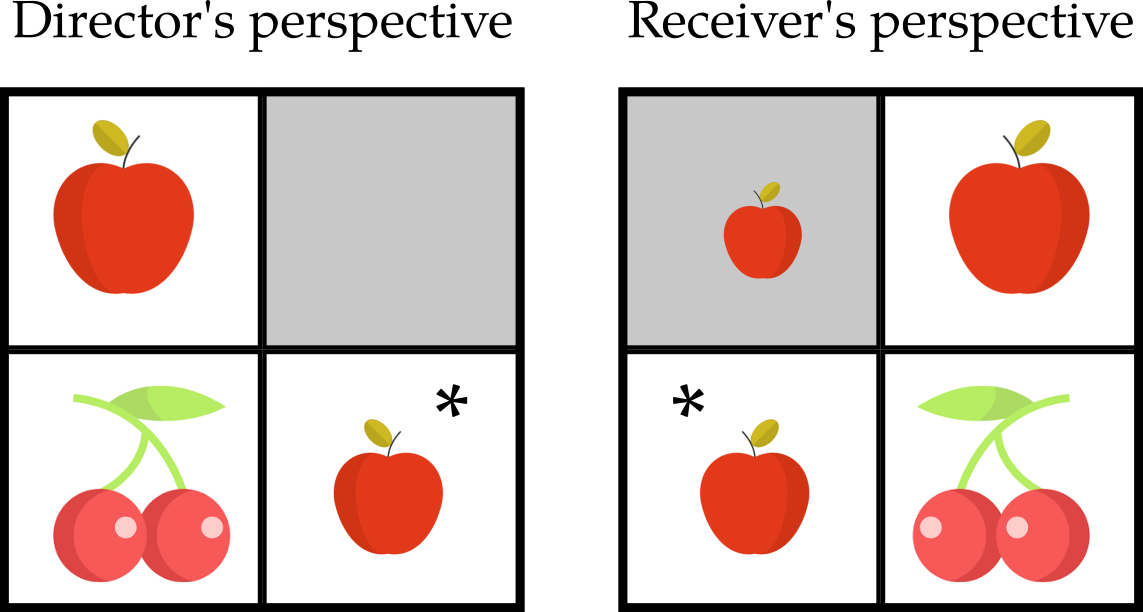
\includegraphics[width=0.5\textwidth]{figures/chapter5/dt_apple.png}
\caption{An example of the perspective difference between the director and the receiver.}
\label{fig:chap5dtapple}
\end{figure}

The director asks the receiver to move some objects by describing them. However, some descriptions of the director will also match other objects ---called competitors--- that are only visible by the receiver. Hence, the receiver must think that the object matching the description cannot be the one referred by the director as they are not aware of it, and find the object matching the description in the director's beliefs. This process must then be maintained all along the interaction as the situation evolves. For example, to designate the starred apple in Figure~\ref{fig:chap5dtapple}, the director may say ``the small apple'', however in the receiver's perspective, directly interpreting this sentence does not result in the starred apple. A decisional process is required, called perspective taking, to decide that the smallest apple in the receiver's perspective cannot be the one designated by the director as they cannot see it, so they are referring to the second smallest (being the smallest in their perspective)

This task is used in psychology to study how perspective-taking is used for communication understanding while performing a task with another agent \cite{keysar2000taking}. Results show that, even if the receiver considered or took a competitor for the first trial, they are able to take the one designated by the director during subsequent trials. This shows that even if participants understand language in an egocentric way, they are able to do perspective-taking to successfully perform the task \cite{keysar2003limits}. 

Even if this task is well known by psychologists, to our knowledge, no robot managed to handle it. A robot that does would prove its architecture being able to maintain self-other distinction of beliefs but also to perform perspective taking on its human partner. We propose a robotic architecture integrating our planner, that is able to handle both side of the director task. Besides, we propose some changes for both the director and receiver roles to be interesting along with planning challenges some modifications of the task can arise.

\subsection{Setup}
The setup we propose is a slight variation of the original director task used in psychology. First, instead of moving objects between compartments, the high level known goal is to remove a subset of the objects in the compartments and to place them in a receiver accessible only area (on top of a table). 


Then, objects are replaced with blocks having four special attributes: their color, the color of their border, the shape drawn on them and the color of this shape. The colors can either be blue or green, and the shapes either a triangle or a circle. This allows for a maximum of ambiguity between the blocks. The used material is presented in Figure~\ref{fig:chap5material}.

\begin{figure}[hbtp]
\centering
\includegraphics[width=\textwidth]{figures/chapter5/material.JPG}
\caption{The material used for the director task. It aims at being simple and cheap to build to encourage the replication of the task.}
\label{fig:chap5material}
\end{figure}

Besides, to make the task interesting for both the director and receiver roles, compartment are not only either fully opened or hiding content from the director, they can also be hiding content from the receiver while being opened towards the director. Thus, not only the receiver must take the perspective of the director to understand the right block, but the director has also to take the perspective of the receiver to make the smallest instruction possible to respect the maxim of quantity~\cite{grice1975logic}. In the example depicted in Figure~\ref{fig:chap5dtpersp}, the minimal sentence to designate the circled block is ``the blue block'', but it requires both agents to perform perspective taking. Indeed, to rule out the distractors (designated with an arrow on the figure), it require to deduce that they cannot have been referred by the other as they are not visible (and to an other extent, not known) by them.

\begin{figure}[hbtp]
\centering
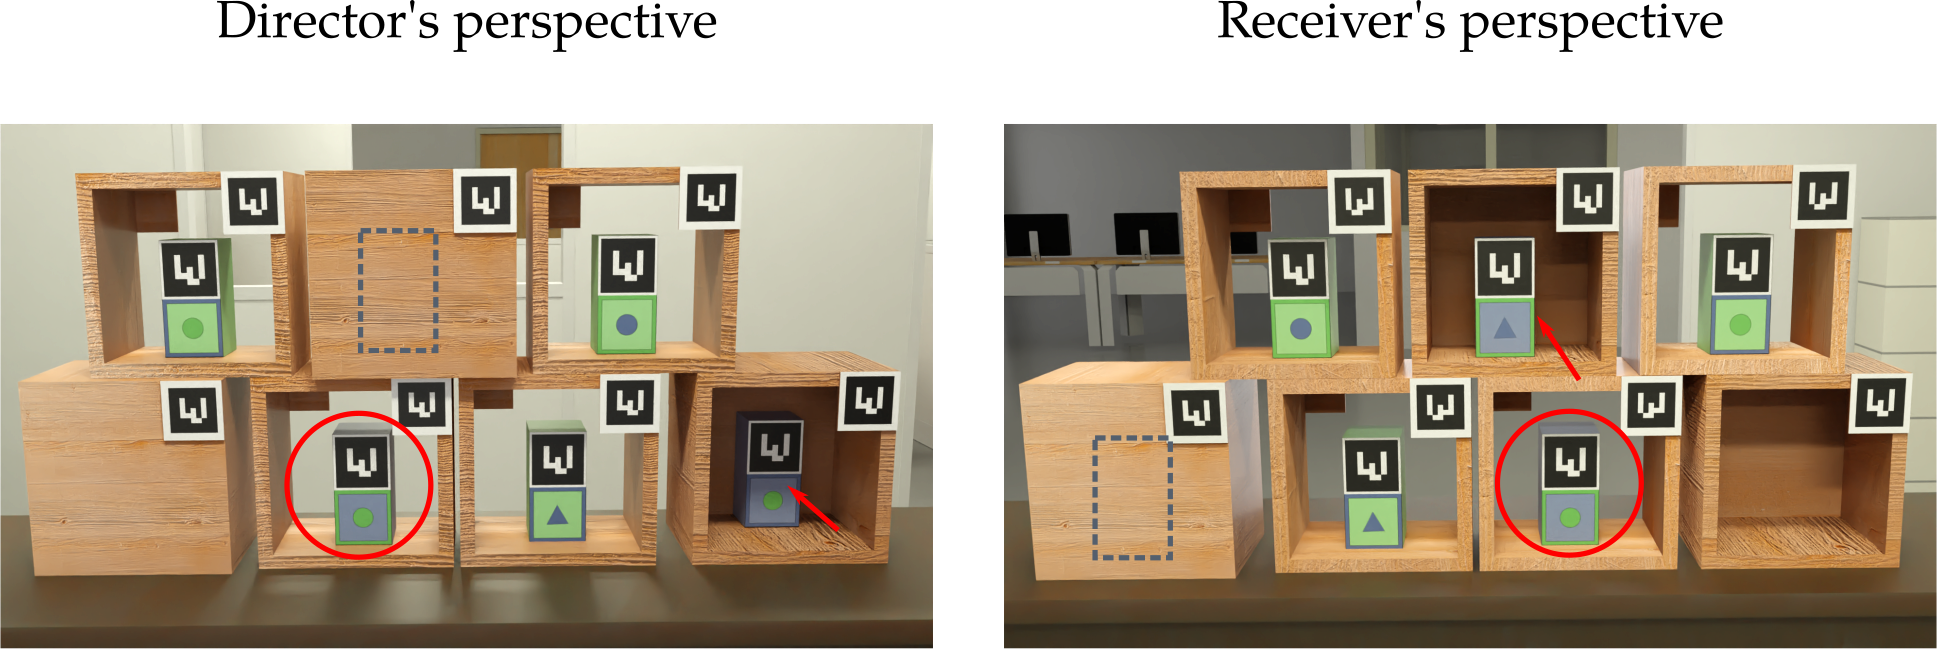
\includegraphics[width=\textwidth]{figures/chapter5/setup.png}
\caption{An example of both the director and receiver perspective in the director task. Here, to designate the circled block the sentence ``the blue block'' is enough as the distractors (designated with red arrows) can be ruled out through perspective taking.}
\label{fig:chap5dtpersp}
\end{figure}

In addition, to increase the number of ambiguous situations, we prohibit the use of geometrical relations during the communications (\textit{e.g.} ``the leftmost block'', ``the block above the green one'') to only allow the use of the block attributes. Likewise, pointing at a block is forbidden.
Finally, every blocks and compartments are equipped with AR-tags (different on each face) allowing the robot to easily detect them and to make an accurate representation of the environment (Figure~\ref{fig:chap5material}).

\subsection{The Robotic Architecture}
The robotic architecture (Figure~\ref{fig:chap5dtarchi} is inspired by the one described by Lemaignan \textit{et al.}~\cite{lemaignan2017artificial} and is composed of several elements.

\begin{figure}[hbtp]
\centering
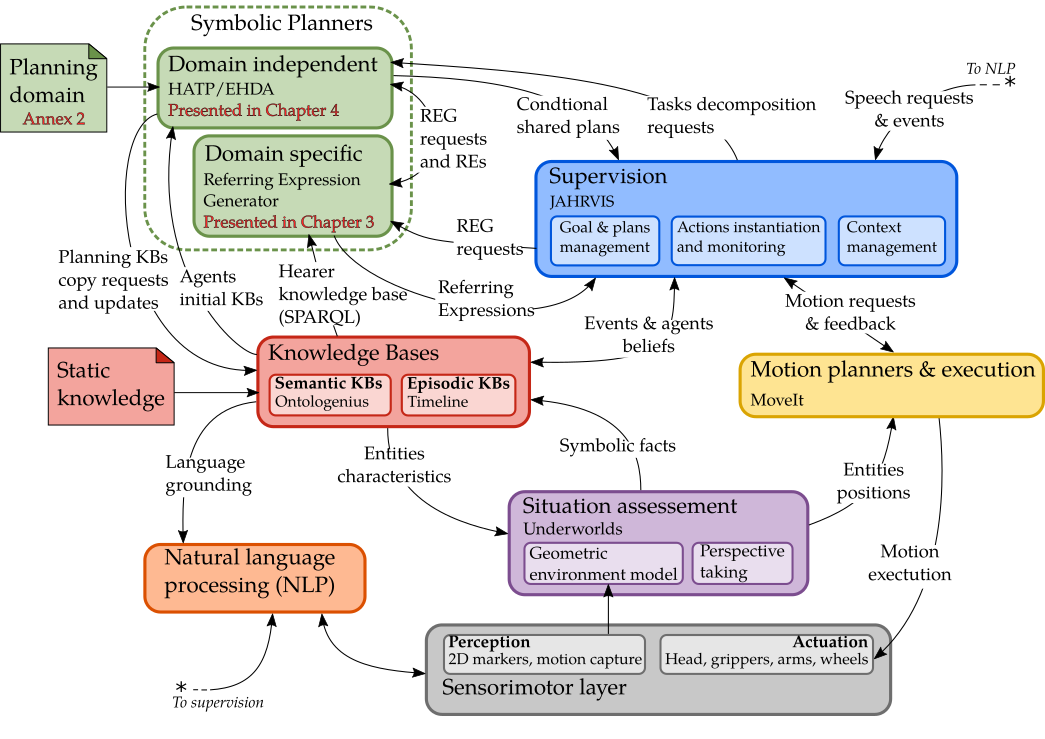
\includegraphics[width=\textwidth]{figures/chapter5/architecture.png}
\caption{The robotic architecture implemented to handle both perspective of the director task. The component circled with a dashed green line are presented in this thesis.}
\label{fig:chap5dtarchi}
\end{figure}

First, the knowledge base chosen is an ontology. As we have shown before, ontologies are more and more common in robotics as they allow for rich and complete reasoning mechanisms and efficient requests of symbolic facts. The software used is \textit{Ontologenius}~\cite{sarthou2019ontologenius}. An ontology is created for the robot ($\robotmodel$, which we use as the true state of the environment) and another one is created for the human ($\humanmodel$) representing the robot estimation of the human knowledge. As stated in the previous chapter, these ontologies can be queried or updated through an efficient low-level API or higher-level \sparql{} queries. The interfaces between the ontologies and our planner are presented in Section~\ref{sec:chap5integratingwithothers}. The ontology is initialized with static facts being (1) the link between each AR-tag and their matching block and compartment, (2) the attributes of each block, (3) the 3D models of each block and compartment.

To gather all the robot sensing data, create a geometric representation of the environment, compute symbolic facts from it for both the robot and the human and update the ontologies with them, a situation assessment component is added to the architecture. This component is based on underwolds~\cite{lemaignan2018underworlds} allowing for modular and reusable reasoners. It first gathers the data from perception algorithm (AR-tags positions for the objects and motion capture for the human), then creates a geometrical scene of the environment. Based on it, the component is able to compute symbolic facts: \textit{isIn}, \textit{isVisibleBy}, \textit{isReachableBy}, \textit{isOnTopOf}; and feed them in real time to the ontology. This component also estimates the geometrical scene viewed and known by the human, computes symbolic facts on it and feed the corresponding ontology.

Then, to be able to give and understand instructions, the REG component presented in the previous chapter is also included. A grammar-based verbalization component allows to transform the generated RE into natural language. Similarly, a natural language request can be interpreted as a \sparql{} query and matched against an ontology.

To orchestrate all the components, the supervision system called JAHRVIS (Joint Action-based Human-aware supeRVISor) is dedicated to manage the interaction. It not only handles the robot actions but also estimates the human mental state, monitors the human actions and manages the communication with them. It manages five facets of the interaction: (1) interactions sessions, (2) communication, (3) human, (4) task and (5) quality of interaction. It is responsible for task planning requests and plan execution and monitoring.

Finally, the task planning component used in this architecture is the one presented in this chapter. Task planning is only required when the robot is the director, since when the robot is receiver it only has to execute commanded instructions. When the robot is the director, the supervision system is given a list of blocks (via their ids) to remove from the shelves. This list is then passed as the goal parameter of a task to decompose to the planner.
The task to decompose is called \verb'clear_blocks' and is filled with a parameter representing the goal and another being the human id. The goal is simply an under specified world state, composed of triplets containing for example \verb'(block_23, isIn, disposalArea)'.
The robot task planning domain ($\robotmodel$) is presented hereafter. 
\begin{itemize}
\item The \verb'clear_blocks' abstract task has only one (recursive) decomposition. The decomposition returns $()$ if the blocks specified in the goal matches the relations also specified in the goal. Otherwise, a REG request is performed for all the misplaced blocks, and the tasks \verb'clear_one_block' and \verb'clear_blocks' are returned, with the easiest block to refer to (\textit{i.e.} lowest RE cost) as parameter of the \verb'clear_one_block' task.
\item The \verb'clear_one_block' task has also only one decomposition returning the primitive task \verb'tell_human_to_clear_block' and the abstract one \verb'wait_for_human_to_clear_block'.
\item The \verb'wait_for_human_to_clear_block' abstract task has only one decomposition. It aims at recursively planning to wait until we planned the human has removed and put the right block away. It recursively decomposes into $()$ if the block passed as argument is in the right place; and returns \verb'wait' and \verb'wait_for_human_to_clear_block' otherwise.
\end{itemize}

The robot primitive tasks are defined as follow:
\begin{itemize}
\item The \verb'tell_human_to_clear_block' primitive task returns $\bot$ if the block specified as parameter is not reachable by the human, or if it is not present in the human beliefs $\humanmodel$. Else, it adds the abstract task \verb'clear_told_block' to the human agenda passing the specified block as parameter and does not update any beliefs.
\item The \verb'wait' primitive task does not update any beliefs.
\end{itemize}

On the human tasks side, we modeled a cooperative human, non declining asked tasks. Thus, the task model is as follows:
\begin{itemize}
\item The abstract task \verb'clear_told_block' has only one decomposition, returning the primitive tasks \verb'pick_block' and \verb'place_block'.
\item The primitive task \verb'pick_block' return $\bot$ if the block passed as parameter is not reachable by the human in their beliefs; and updates the beliefs of all the agents in the room with the human holding the block otherwise.
\item The primitive task \verb'place_block' return $\bot$ if the human is not carrying anything; else it updates the beliefs of all the agents in the room with the block being placed in the area specified as parameter, and the human not holding anything.
\end{itemize}

In the domain described previously, we compute in the abstract task the least costly block to refer to to decompose the task. This greedy approach can be used because we remove the block during the task. The referring cost of blocks thus can only decrease at each iteration of the task. However, it would be completely different if some blocks were to be added to the shelf along with others to remove. There, our greedy approach would not work as an not costly action would make future actions more costly leading to an sub-optimal plan. Another approach could be to have the decomposition of \verb'clear_blocks' to return all the orders of the block removing instructions to explore.

In the proposed version of the director task, only the cube order can be planned. Thus, in the following subsection, we propose slight variations of the task increasing the planning complexity and interest, along with some possible modeling directions to overcome these challenges.

\begin{figure}[hbtp]
\centering
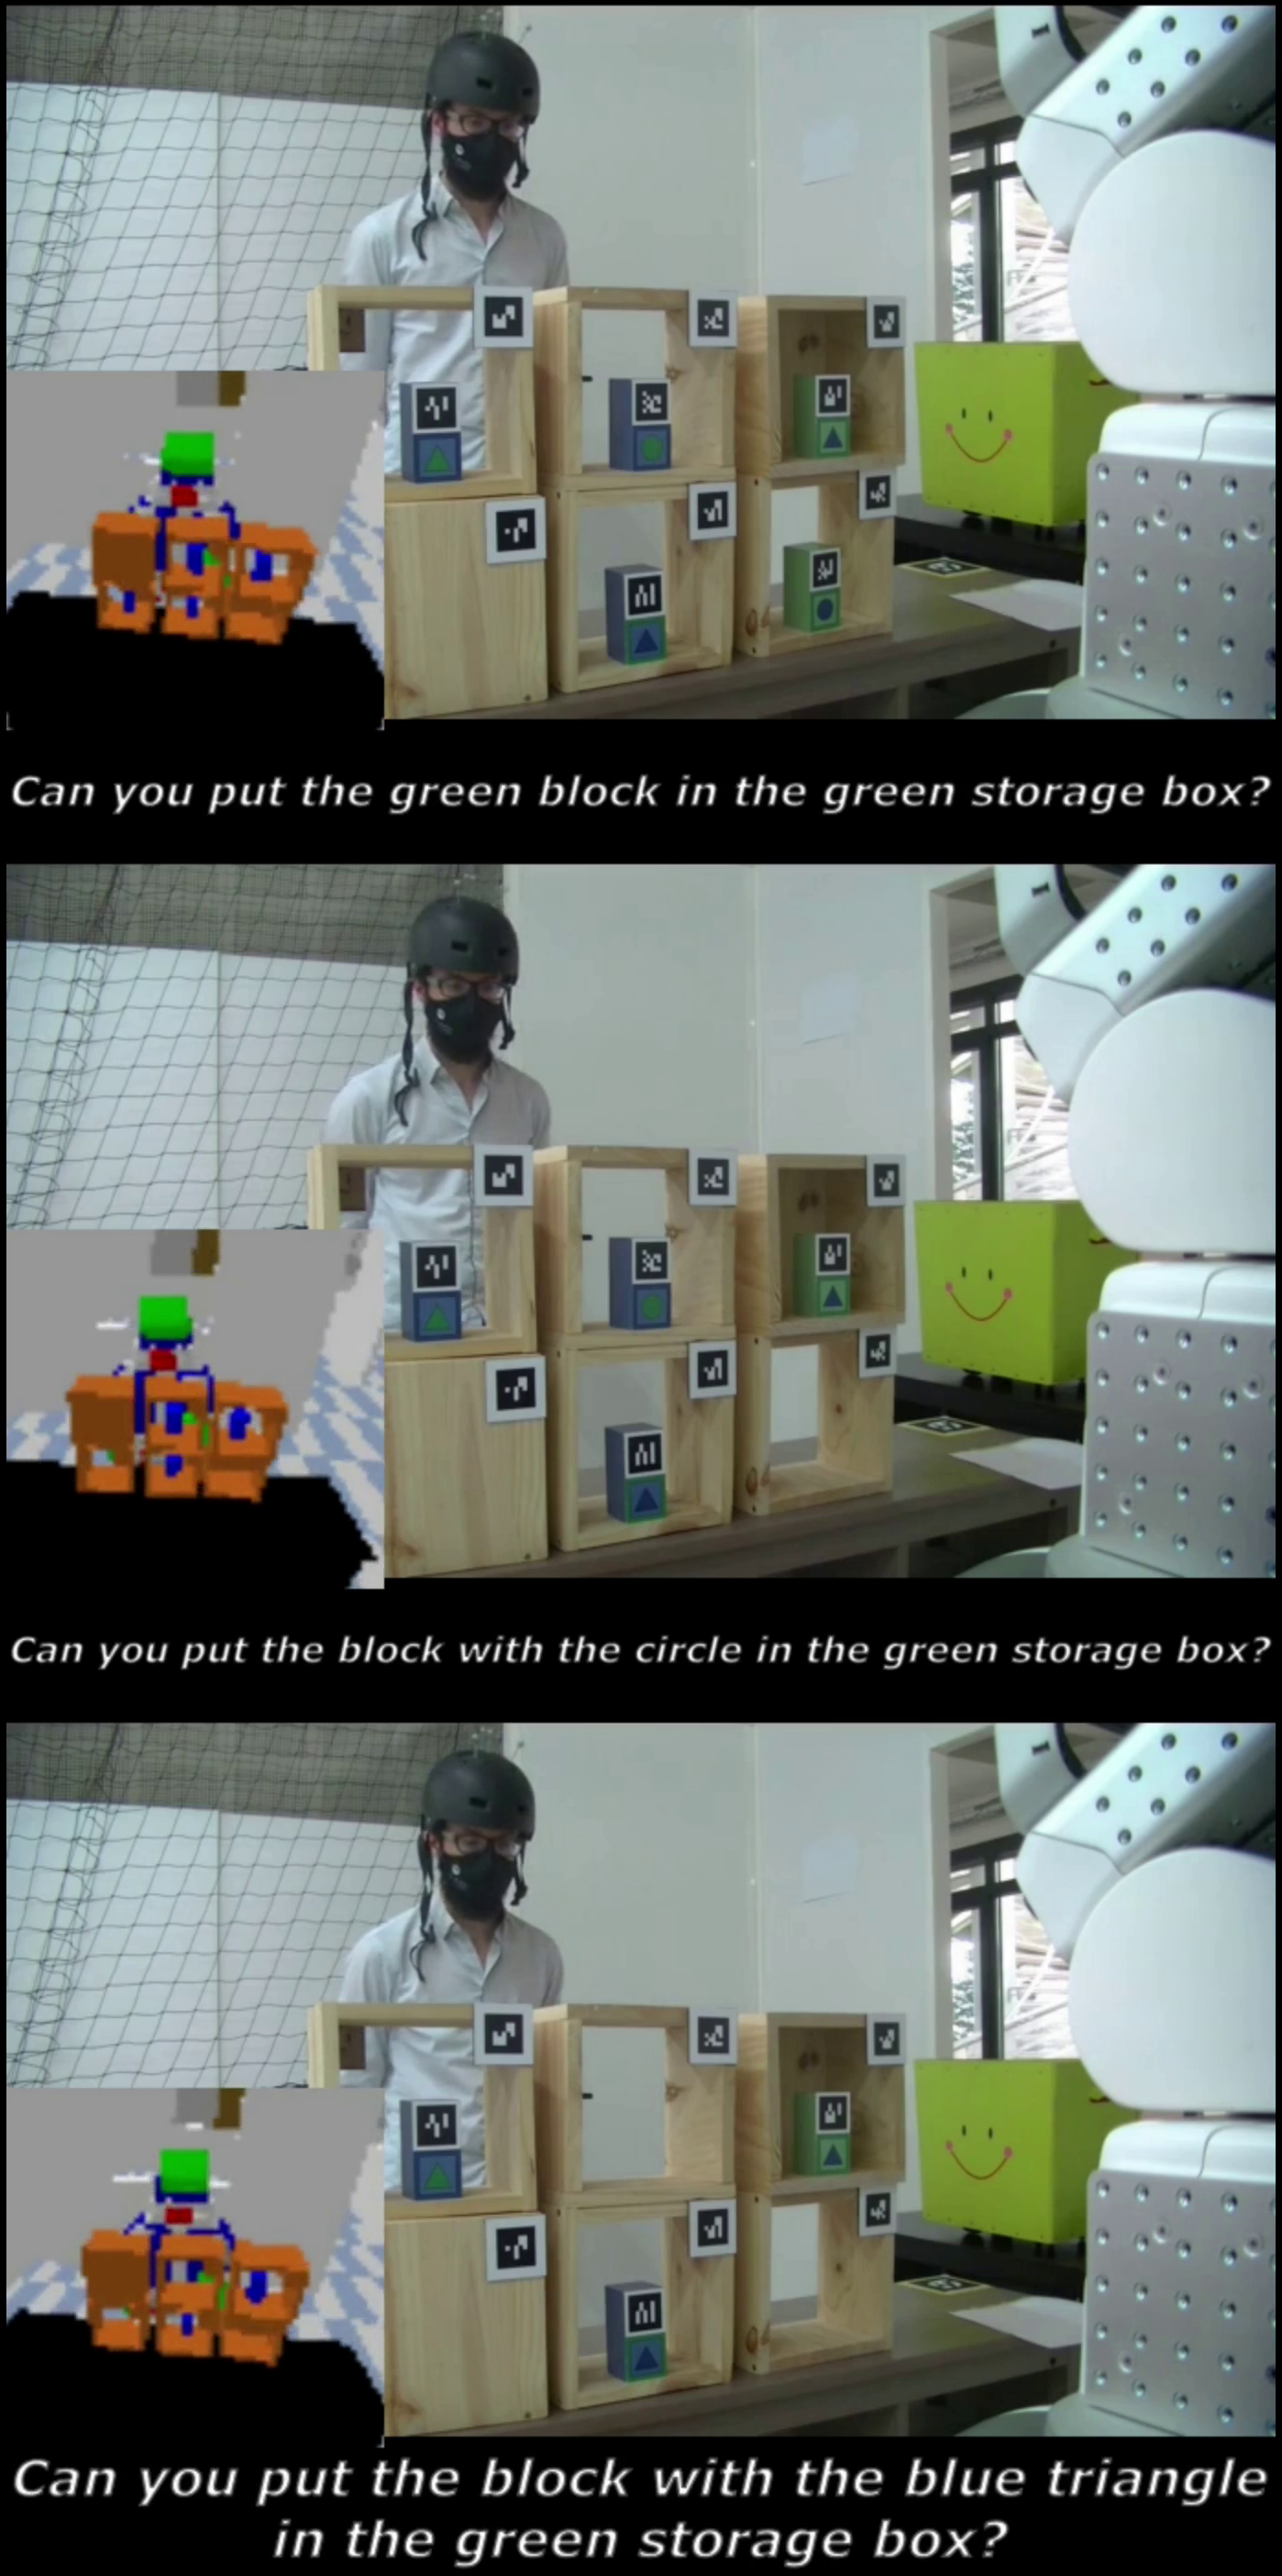
\includegraphics[width=0.5\textwidth]{figures/chapter5/dt_demo.png}
\caption{The director task handled by an autonomous PR2 robot in the director role. The computed human perspective is displayed in the bottom left hand corner of picture. The robot said sentence is printed under each picture.}
\label{fig:chap5dtdemodirector}
\end{figure}

A video presenting the architecture used in a real interaction to both tackle the director and the receiver perspective is available at \url{https://cloud.laas.fr/index.php/s/kx6m67rt5n8bvky}. When the robot is director, thanks to the planning scheme presented in this thesis, it is able to compute the minimal referring expression to designate the blocks while accounting for the human perspective. Moreover, it gives the instructions in the order minimizing the complexity of referring expression at each step (Figure\ref{fig:chap5dtdemodirector}). Finally, the robot is also able to handle the receiver role  by taking the human perspective when it processes their instructions. Moreover, using the REG algorithm presented in Chapter~\ref{chapter:comm}, if the human instruction is detected as being ambiguous (multiple entities matching the \sparql{} built from sentence he said), the robot is able to ask the right questions to find the right entity (Figure~\ref{fig:chap5dtdemoreceiver}). For each matching entity, a REG is performed with the relations found in the human utterance (and used in the \sparql{} query) are given as context. This allows to find the missing relations disambiguating the entities. The supervision then use the REs returned to ask ``Do you mean \textit{RE1} or \textit{RE2}?'', and keep the previous context to add it to the \sparql{} query built with the human answer.

\begin{figure}[hbtp]
\centering
\includegraphics[width=\textwidth]{figures/chapter5/dt_demoreceiver.png}
\caption{The director task handled by an autonomous PR2 robot in the receiver role. The robot is able to take the perspective of the human to understand his instructions, and can ask pertinent questions if the human instruction is ambiguous. Please note that some shapes on the blocks have been redrawn on the picture to enhance the contrast and improve its readability.}
\label{fig:chap5dtdemoreceiver}
\end{figure}

\subsection{Challenges for Planning}
To spice up the planning challenge in the director task, we propose some extensions to the presented task.
First, by adding blocks with identical visual features to the shelf, and asking to remove a precise one of them, we introduce situations where verbal communication (and REG) is not enough to refer to a block. To solve this problem, we could for example add a decomposition to \verb'clear_one_block'. In this decomposition, we could have the robot moving one distractor of the REG in a non visible compartment to be able to refer to the intended block. The planner would then have to balance between making the referring easier by moving a block before giving the instruction and giving a long and complex instruction (when feasible).

With the same scenario, using the REG extension presented in the previous chapter, allowing the RE to contain relations to past common actions, we could introduce another way for the robot to refer to a block. The planner would need to balance previous communication means with creating a unique past experience with a block to easily refer to it (\textit{e.g.} ``the blue block that I just moved'').

Besides, we can add multiple distinct disposal areas for blocks. The director would then have to instruct the receiver not only the block to pick but also which area they have to place it in. Furthermore, we could also add a decomposition where the robot ask to pick an under specified block, ensuring that all the matching ones need to be removed, and plan for all the possible blocks picked by the human matching this description. Depending on the block picked, it would be planned to ask to place the cube in its corresponding area. This may result in a better efficiency as it would lead to less complex referring expressions.

Finally, performing this task will necessarily bring errors, either from the human (\textit{e.g.} the wrong block may be picked) or the robot (\textit{e.g.} a block may fail to be picked). Even if some errors can be planned for (\textit{e.g.} modeling all the blocks the human can pick and planning accordingly) doing so for all the possible contingencies is not possible. Therefore, a strong link with supervision must be envisioned as it will ask for replanning. Replanning is not as simple as passing the current state and the same goal and starting the process all over again, since some task decomposition may have been executed partially and cannot be changed in the replanning process.

% Code words + Multiple sessions
% Communicating about multiple blocks at once

\section{Conclusion}
In this chapter, we showed how the task planning scheme presented earlier can be integrated in a robotic architecture. It can use larger knowledge bases to initialize the robot and the human beliefs, interface with domain-specific planners such as the REG approach presented in Chapter~\ref{chapter:comm} and provide a service mechanism of ROS for the supervision to make planning requests.

Finally, an easy to reproduce yet challenging task for HRI was presented, along with a robotic architecture to handle this task. The planning scheme presented in Chapter~\ref{chapter:doublehtn} was used when the robot is director to plan for the sequence of actions minimizing the communication complexity, and the REG component presented in Chapter~\ref{chapter:comm} was used for both the director and receiver role to either find referring expressions for objects to be included in the instructions or to refine a human instruction when it has been detected as ambiguous.

\ifdefined\included
\else
\bibliographystyle{acm}
\bibliography{These}
\end{document}
\fi
